\subsection{Towards Ductile Fracture}
\subsectioncover

\begin{frame}
  \vspace{-1.5em}
  \begin{columns}
    \begin{column}{0.2\textwidth}
      \vspace{-1em}
      \begin{figure}
        \centering
        \begin{subfigure}{\textwidth}
          \centering
          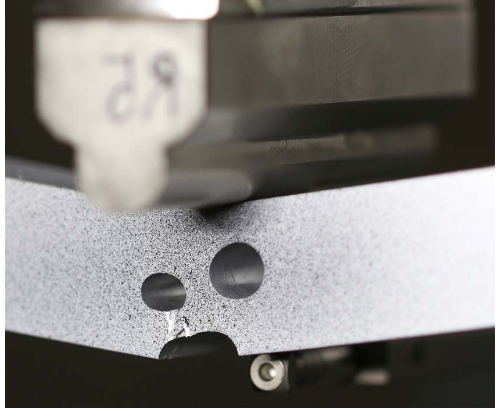
\includegraphics[width=\textwidth]{Chapter345/figures/3pb_real_crack}
        \end{subfigure}
        \begin{subfigure}{\textwidth}
          \centering
          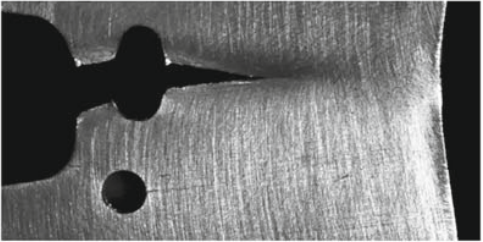
\includegraphics[width=\textwidth]{Chapter345/figures/SFC_schematics}
        \end{subfigure}
        \begin{subfigure}{\textwidth}
          \centering
          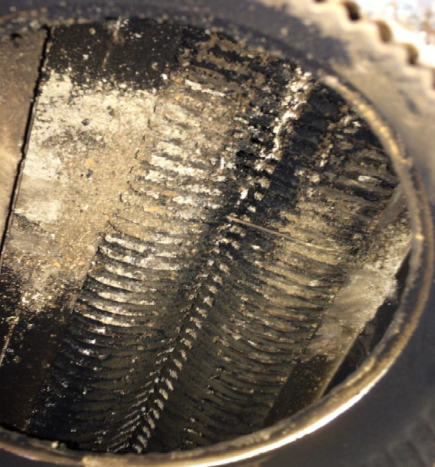
\includegraphics[width=\textwidth]{Chapter1/figures/spallation}
        \end{subfigure}
      \end{figure}
    \end{column}
    \begin{column}{0.8\textwidth}
      \vspace{1em}
      
      There exist many approaches to modeling plasticity in the context of phase-field fracture \cite{alessi_gradient_2014, alessi_gradient_2015, alessi_coupling_2018, ambati_phase-field_2015, ambati2016phase, miehe_phase_2016, borden2016phase, borden_phase-field_2017}.
      
      \bigskip
      \pause
      
      How to best design the \textcolor{peggyblue}{coupling} between plasticity and fracture remains an open question. Some challenges/issues:
      \begin{itemize}
        \item<3-> Fracture tends to propagate along the plastic zone.
        
        \item<4-> Most existing models
        \begin{itemize}
          \item<4-> are not variational,
          \item<5-> require \textcolor{peggyblue}{re-calibration} of material parameters,
          \item<6-> result in \textcolor{peggyblue}{regularization-dependent} response.
        \end{itemize}
        \includegraphics<5>{Chapter345/figures/bad_alpha}
        \includegraphics<6>[width=0.3\textwidth]{Chapter345/figures/R_curve_threshold}
        \item<7-> How much plastic work contributes to \textcolor{peggyblue}{fracture evolution}?
        \item<8-> How much plastic work converts to \textcolor{peggyblue}{heat generation}?
      \end{itemize}
      
      \bigskip
      
      \only<9->{
        \begin{block}{}
          \centering
          \vspace{1em}
          All of the issues above can be addressed by the proposed framework \\
          (with proper constitutive choices).
          \vspace{1em}
        \end{block}
      }
    \end{column}
  \end{columns}
\end{frame}

\begin{frame}
  \vspace{-1.5em}
  \begin{block}{}
    \begin{align*}
      L = \int\limits_{\body_0} \left[ \textcolor<1>{red}{\dot{\psi}^e} + \textcolor<2>{red}{{\psi^e}^*} + (1-\tqf) \textcolor<4>{red}{\dot{\psi}^p} + \tqf \textcolor<4>{red}{{\psi^p}^*} + \textcolor<5>{red}{\dot{\psi}^f} + \textcolor<5>{red}{{\psi^f}^*} - T\dot{s} - \textcolor<6>{red}{\chi} \right] \diff{V} - \mathcal{P}^\text{ext}, \\
      \textcolor<3,5>{red}{\text{subject to } \bfL(\bfZ) \dot{\bfZ} = \bs{0}}.
    \end{align*}
  \end{block}
  
  \begin{overlayarea}{\textwidth}{0.4\textwidth}
    \only<1>{
      \begin{columns}[T]
        \begin{column}{0.5\textwidth}
          Option 1 (Compressible Neo-Hookean):
          \begin{align*}
            \psi^e               = & \ g^e \psi^e_\activepart + \psi^e_\inactivepart,                                                              \\
            \psi^e_\activepart   = & \ \mathbb{H}_1(J)\left\{ \dfrac{1}{2}K\left[ \dfrac{1}{2}(J^2-1) - \ln(J) \right] \right\}                    \\
                                   & \ + \dfrac{1}{2}G\left( \overbar{\bfC}:{\bfC^p}^{-1} - 3 \right),                                             \\
            \psi^e_\inactivepart = & \ \left( 1-\mathbb{H}_1(J) \right) \left\{ \dfrac{1}{2}K\left[ \dfrac{1}{2}(J^2-1) - \ln(J) \right] \right\}. 
          \end{align*}
        \end{column}
        \begin{column}{0.5\textwidth}
          Option 2 (Hencky):
          \begin{align*}
            \psi^e               & =  g^e \psi^e_\activepart + \psi^e_\inactivepart,                                     \\
            \psi^e_\activepart   & = \dfrac{1}{2} K \macaulay{\tr(\strain^e)}_+^2 + G \dev{\strain^e} : \dev{\strain^e}, \\
            \psi^e_\inactivepart & = \dfrac{1}{2} K \macaulay{\tr(\strain^e)}_-^2,                                       \\
            \strain^e            & = \frac{1}{2} \ln\left( \bfC^e \right).                                               
          \end{align*}
        \end{column}
      \end{columns}
    }
    
    \only<2>{
      \begin{columns}
        \begin{column}{0.5\textwidth}
          Newtonian viscosity:
          \begin{align*}
            {\psi^e}^* & = g^e J \left[ \dfrac{1}{2}\zeta \tr(\bfd)^2 + \eta \bfd:\bfd \right], \\
            \bfd       & = \sym\left( \dot{\defgrad}\defgrad^{-1} \right).                      
          \end{align*}
        \end{column}
      \end{columns}
    }
    
    \only<3>{
      \begin{columns}[T]
        \begin{column}{0.4\textwidth}
          Flow rule constraints:
          \begin{align*}
            \tr\left( \dot{\defgrad}^p{\defgrad^p}^{-1} \right) = 0, \\
            \norm{\dot{\defgrad}^p{\defgrad^p}^{-1}}^2 - \frac{3}{2} \abs{\epdot}^2 = 0.
          \end{align*}
        \end{column}
        \begin{column}{0.6\textwidth}
          \begin{remark}[Flow rule]
            It recovers the Prandtl-Reuss flow rule:
            \begin{align*}
              \dot{\defgrad}^p{\defgrad^p}^{-1} = \epdot \bfN^p, \quad \bfN^p = \sqrt{\dfrac{3}{2}}\dfrac{\dev(\bfM)}{\norm{\dev(\bfM)}},
            \end{align*}
            and the loading/unloading conditions:
            \begin{align*}
               & \phi^p \leqslant 0, \quad \epdot \geqslant 0, \quad \phi^p\epdot = 0,                       \\
               & \phi^p = \norm{\dev(\bfM)} - \sqrt{\dfrac{2}{3}} \left( Y^\text{eq} + Y^\text{vis} \right). 
            \end{align*}
          \end{remark}
        \end{column}
      \end{columns}
    }
    
    \only<4>{
      \begin{columns}[T]
        \begin{column}{0.5\textwidth}
          Option 1 (Linear hardening):
          \begin{align*}
            \psi^p     & = g^p \left( \sigma_y \ep + \dfrac{1}{2} H \ep^2 \right), \\
            {\psi^p}^* & = g^p (\sigma_y + H \ep) \epdot.                          
          \end{align*}
          Option 2 (Power-law hardening):
          \begin{align*}
            \psi^p     & = g^p \dfrac{n}{n+1} \sigma_y \epsilon_0 \left[ \left( 1 + \dfrac{\ep}{\epsilon_0} \right)^{(n+1)/n} - 1 \right], \\
            {\psi^p}^* & = g^p \sigma_y \left( 1 + \dfrac{\ep}{\epsilon_0} \right)^{1/n} \epdot.                                           
          \end{align*}
        \end{column}
        \begin{column}{0.5\textwidth}
          Option 3 (Perfect plasticity with thermal softening):
          \begin{align*}
            \psi^p     & = g^p \sigma_y^T \ep, \quad {\psi^p}^* = g^p \sigma_y^T \epdot, \\
            \sigma_y^T & = \dfrac{\sigma_0}{\exp\left( -\dfrac{Q}{RT} \right)}           
          \end{align*}
          \begin{remark}[The Taylor-Quinney factor]
            Due to thermal softening (option 3), to get an increase in temperature from plastic dissipation:
            \begin{align*}
              \dfrac{Q}{Q+RT} \leqslant \tqf \leqslant 1.
            \end{align*}
          \end{remark}
        \end{column}
      \end{columns}
    }
    
    \only<5>{
      \begin{columns}[T]
        \begin{column}{0.5\textwidth}
          Fracture energy density:
          \begin{align*}
            \psi^f = \dfrac{\Gc}{c_0l}\left( C \alpha + l^2 \grad d \cdot \grad d \right).
          \end{align*}
          Viscous regularization and coalescence dissipation:
          \begin{align*}
            {\psi^f}^* = & \ \dfrac{1}{2} v \dot{d}^2 + (1-C) \dfrac{\Gc}{c_0 l}\alpha_{, d}\dot{d}                  \\
                         & \ - (1-\beta)\dfrac{\Gc}{c_0l}\alpha_{,d}\left( 1-e^{-\ep/\varepsilon_0} \right)\dot{d} . 
          \end{align*}
          Irreversibility constraint:
          \begin{align*}
            \dot{d} \geqslant 0.
          \end{align*}
        \end{column}
        \begin{column}{0.5\textwidth}
          \begin{remark}
            The contributions from plasticity is clear in the fracture envelope:
            \begin{align*}
              v\dot{d}      & =\divergence \dfrac{2\Gc l}{c_0} \grad d - \left( \dfrac{\widehat{\Gc}}{c_0 l}\alpha_{,d} + \psi^d \right), \\
              \psi^d        & = \psi^e_{,d} + (1-\tqf) \psi^p_{,d},                                                                       \\
              \widehat{\Gc} & = g^c \Gc, \quad g^c = 1-(1-\beta)\left( 1-e^{-\ep/\varepsilon_0} \right),                                  
            \end{align*}
          \end{remark}
          \begin{remark}
            To satisfy the second law: $0 < C \leqslant \beta$.
          \end{remark}
        \end{column}
      \end{columns}
    }
    
    \only<6>{
      \begin{columns}[T]
        \begin{column}{0.5\textwidth}
          Fourier potential:
          \begin{align*}
            \chi & = \dfrac{1}{2}\kappa\btg\cdot\btg, \\
            \btg & = - \grad T / T.                   
          \end{align*}
          \begin{remark}
            The heat conduction equation can be written as
            \begin{align*}
              \rho_0c_v\dot{T} & = \rho_0 q + \divergence \kappa \grad T + \delta + \delta_T,                 \\
              \delta           & = \bfP^\text{vis}:\dot{\defgrad} + Y^\text{vis}\epdot + f^\text{vis}\dot{d}, \\
              \delta_T         & = -g^p (1-\tqf) \dfrac{Q}{RT} \sigma_y^T\epdot.                              
            \end{align*}
          \end{remark}
        \end{column}
      \end{columns}
    }
  \end{overlayarea}
\end{frame}

\begin{frame}
  \begin{columns}[T]
    \begin{column}{0.7\textwidth}
      \vspace{3em}
      How to best design the coupling between plasticity and fracture remains an open question. Some challenges/issues:
      \begin{itemize}
        \item \sout<2->{Fracture tends to propagate along the plastic zone.}
        \item \sout<7->{Most existing models}
              \begin{itemize}
                \item \sout<3->{are not variational,}
                \item \sout<5->{require re-calibration of material parameters,}
                \item \sout<7->{result in regularization-dependent response.}
              \end{itemize}
        \item \sout<8->{How much plastic work contributes to fracture evolution?}
        \item \sout<8->{How much plastic work converts to heat generation?}
      \end{itemize}
    \end{column}
    \begin{column}{0.3\textwidth}
      \vspace{-1.5em}
      \only<4>{
        \begin{figure}
  \centering
  \begin{subfigure}{\textwidth}
    \centering
    \begin{tikzpicture}
      \begin{axis}[
          colormap/jet,
          cycle list={[of colormap,samples of colormap=4]},
          width=\textwidth,
          height=\textwidth,
          xmin=0,
          ymin=0,
          ymax=1.6,
          xlabel=$\varepsilon$,ylabel=$\sigma/\sigma_y$,
          scaled x ticks=false,
          yticklabel style={
              /pgf/number format/fixed,
              /pgf/number format/precision=2
            },
          xticklabel style={
              /pgf/number format/fixed,
              /pgf/number format/precision=2
            },
          legend style={
              at={(0.05,0.98)},
              anchor=north west,
              nodes={scale=0.5, transform shape},
              fill=none,
              draw=none,
              cells={align=left}
            },
          legend cell align={left},
          every axis plot/.append style={thick,no marks}
        ]
        \addplot +[black] table[x expr=\thisrowno{1},y expr=\thisrowno{0}/320,col sep=comma]{Chapter345/data/homogenized_EP.csv};
        \addplot table[x expr=\thisrowno{3},y expr=\thisrowno{2}/320,col sep=comma]{Chapter345/data/homogenized_EPPD_xi_0_psic_1_a_250_R_4.csv};
        \addplot table[x expr=\thisrowno{3},y expr=\thisrowno{2}/320,col sep=comma]{Chapter345/data/homogenized_EPPD_xi_0_psic_2_a_250_R_4.csv};
        \addplot table[x expr=\thisrowno{3},y expr=\thisrowno{2}/320,col sep=comma]{Chapter345/data/homogenized_EPPD_xi_0_psic_3_a_250_R_4.csv};
        \addplot table[x expr=\thisrowno{3},y expr=\thisrowno{2}/320,col sep=comma]{Chapter345/data/homogenized_EPPD_xi_0_psic_4_a_250_R_4.csv};
        \draw[dashed, thick] (0,1) -- (0.06,1);
        \legend{no fracture, $\psi_cc_0a/\Gc=0.005$, $\psi_cc_0a/\Gc=0.010$, $\psi_cc_0a/\Gc=0.015$, $\psi_cc_0a/\Gc=0.019$}
      \end{axis}
    \end{tikzpicture}
  \end{subfigure}
  
  \begin{subfigure}{\textwidth}
    \centering
    \begin{tikzpicture}
      \begin{axis}[
          colormap/jet,
          cycle list={[of colormap,samples of colormap=4]},
          width=\textwidth,
          height=\textwidth,
          xmin=0,
          ymin=0,
          ymax=1.6,
          xlabel=$\varepsilon$,ylabel=$\sigma/\sigma_y$,
          scaled x ticks=false,
          yticklabel style={
              /pgf/number format/fixed,
              /pgf/number format/precision=2
            },
          xticklabel style={
              /pgf/number format/fixed,
              /pgf/number format/precision=2
            },
          legend style={
              at={(0.05,0.98)},
              anchor=north west,
              nodes={scale=0.5, transform shape},
              fill=none,
              draw=none,
              cells={align=left}
            },
          legend cell align={left},
          every axis plot/.append style={thick,no marks}
        ]
        \addplot +[black] table[x expr=\thisrowno{1},y expr=\thisrowno{0}/320,col sep=comma]{Chapter345/data/homogenized_EP.csv};
        \addplot table[x expr=\thisrowno{3},y expr=\thisrowno{2}/320,col sep=comma]{Chapter345/data/homogenized_EPD_xi_1_psic_0.75_a_2500_R_4.csv};
        \addplot table[x expr=\thisrowno{3},y expr=\thisrowno{2}/320,col sep=comma]{Chapter345/data/homogenized_EPD_xi_1_psic_0.77_a_2500_R_4.csv};
        \addplot table[x expr=\thisrowno{3},y expr=\thisrowno{2}/320,col sep=comma]{Chapter345/data/homogenized_EPD_xi_1_psic_0.79_a_2500_R_4.csv};
        \addplot table[x expr=\thisrowno{3},y expr=\thisrowno{2}/320,col sep=comma]{Chapter345/data/homogenized_EPD_xi_1_psic_0.81_a_2500_R_4.csv};
        \draw[dashed, thick] (0,1) -- (0.06,1);
        \legend{no fracture, $\psi_cc_0a/\Gc=0.036$, $\psi_cc_0a/\Gc=0.037$, $\psi_cc_0a/\Gc=0.038$, $\psi_cc_0a/\Gc=0.039$}
      \end{axis}
    \end{tikzpicture}
  \end{subfigure}
\end{figure}

      }
      \only<6>{
        \begin{figure}
  \centering
  \begin{subfigure}{\textwidth}
    \centering
    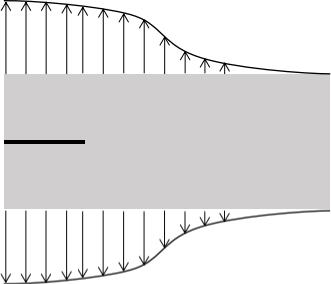
\includegraphics[width=0.75\textwidth]{Chapter345/figures/surfing_bc}
  \end{subfigure}
  
  \vspace{0.1\textwidth}
  
  \begin{subfigure}{\textwidth}
    \centering
    \begin{tikzpicture}
      \begin{axis}[
          colormap/jet,
          cycle list={[of colormap,samples of colormap=8]},
          width=\textwidth,
          height=\textwidth,
          xlabel=$\Delta a / r_p$,ylabel=$J / \Gc$,
          xmin=0,
          ymin=0,
          legend style={at={(0.95,0.05)},anchor=south east},
          legend style={nodes={scale=0.5, transform shape}},
          legend cell align={left},
          every axis plot/.append style={no marks}
        ]
        \addplot table[x expr=(\thisrowno{2}*2-1.7989255734091782)/0.05996418578030594, y expr=\thisrowno{1}*2/2.7, col sep=comma]{Chapter345/data/R_1.csv};
        \addplot table[x expr=(\thisrowno{2}*2-1.6190330160682607)/0.05996418578030594, y expr=\thisrowno{1}*2/2.7, col sep=comma]{Chapter345/data/R_0.9.csv};
        \addplot table[x expr=(\thisrowno{2}*2-1.4391404587273429)/0.05996418578030594, y expr=\thisrowno{1}*2/2.7, col sep=comma]{Chapter345/data/R_0.8.csv};
        \addplot table[x expr=(\thisrowno{2}*2-1.2592479013864248)/0.05996418578030594, y expr=\thisrowno{1}*2/2.7, col sep=comma]{Chapter345/data/R_0.7.csv};
        \addplot table[x expr=(\thisrowno{2}*2-1.079355344045507)/0.05996418578030594, y expr=\thisrowno{1}*2/2.7, col sep=comma]{Chapter345/data/R_0.6.csv};
        \addplot table[x expr=(\thisrowno{2}*2-0.8994627867045891)/0.05996418578030594, y expr=\thisrowno{1}*2/2.7, col sep=comma]{Chapter345/data/R_0.5.csv};
        \addplot table[x expr=(\thisrowno{2}*2-0.7195702293636714)/0.05996418578030594, y expr=\thisrowno{1}*2/2.7, col sep=comma]{Chapter345/data/R_0.4.csv};
        \addplot table[x expr=(\thisrowno{2}*2-0.5396776720227535)/0.05996418578030594, y expr=\thisrowno{1}*2/2.7, col sep=comma]{Chapter345/data/R_0.3.csv};
        \legend{$l/r_p=1$, $l/r_p=0.9$, $l/r_p=0.8$, $l/r_p=0.7$, $l/r_p=0.6$, $l/r_p=0.5$, $l/r_p=0.4$, $l/r_p=0.3$}
      \end{axis}
    \end{tikzpicture}
  \end{subfigure}
\end{figure}

      }
    \end{column}
  \end{columns}
\end{frame}

\begin{frame}
  \begin{columns}[T]
    \begin{column}{0.6\textwidth}
      \vspace{-1em}
      \begin{figure}
        \centering
        \begin{subfigure}{0.32\linewidth}
          \centering
          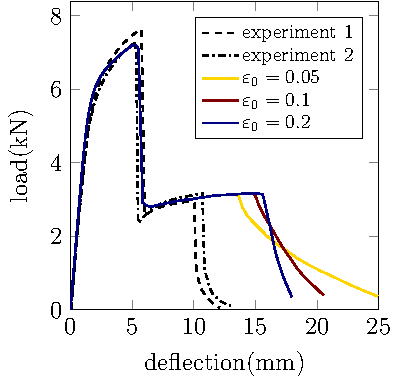
\includegraphics[width=0.8\textwidth]{Chapter345/figures/Chapter5-3pb-load_deflection-constant_beta}
        \end{subfigure}
        \begin{subfigure}{0.32\linewidth}
          \centering
          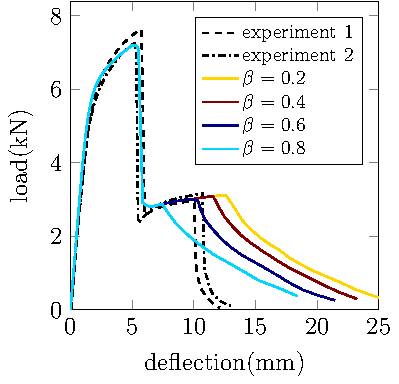
\includegraphics[width=0.8\textwidth]{Chapter345/figures/Chapter5-3pb-load_deflection-constant_e0}
        \end{subfigure}
        \begin{subfigure}{0.32\linewidth}
          \centering
          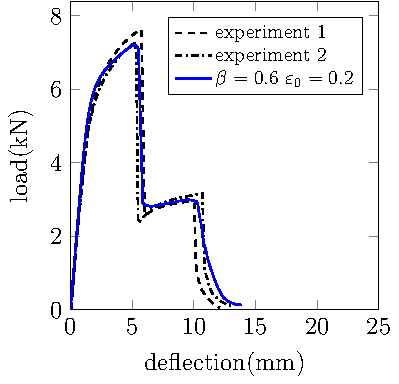
\includegraphics[width=0.8\textwidth]{Chapter345/figures/Chapter5-3pb-load_deflection_tuned}
        \end{subfigure}
        
        \vspace{0.5em}
        
        \begin{subfigure}{0.45\textwidth}
          \centering
          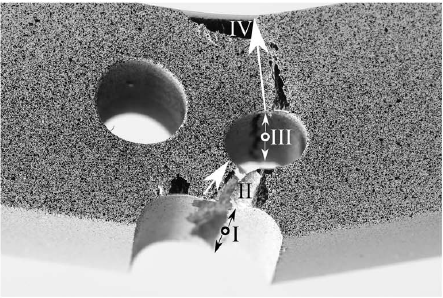
\includegraphics[width=0.7\textwidth,scale=0.5]{Chapter345/figures/1234}
        \end{subfigure}
        \only<1>{
          \begin{subfigure}{0.45\textwidth}
            \centering
            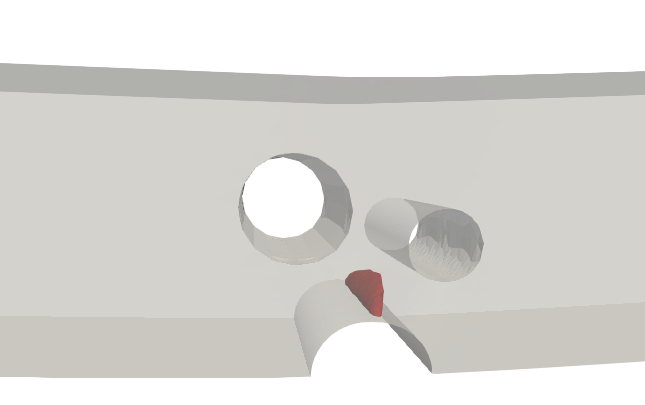
\includegraphics[width=0.7\textwidth]{Chapter345/figures/I}
          \end{subfigure}
        }
        \only<2>{
          \begin{subfigure}{0.45\textwidth}
            \centering
            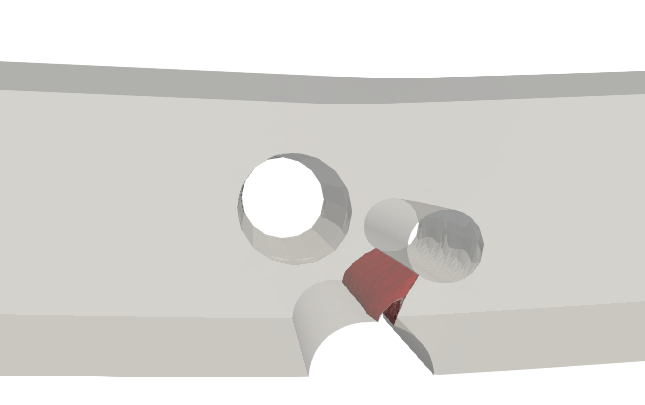
\includegraphics[width=0.7\textwidth]{Chapter345/figures/II}
          \end{subfigure}
        }
        \only<3>{
          \begin{subfigure}{0.45\textwidth}
            \centering
            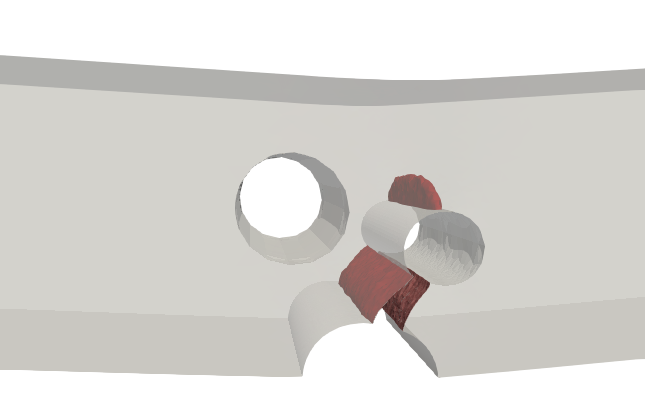
\includegraphics[width=0.7\textwidth]{Chapter345/figures/III}
          \end{subfigure}
        }
        \only<4>{
          \begin{subfigure}{0.45\textwidth}
            \centering
            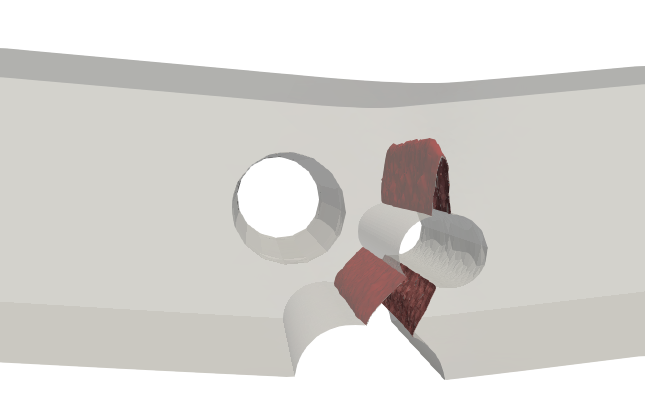
\includegraphics[width=0.7\textwidth]{Chapter345/figures/IV}
          \end{subfigure}
        }
        
        \vspace{0.5em}
        
        \begin{subfigure}[b]{0.45\textwidth}
          \centering
          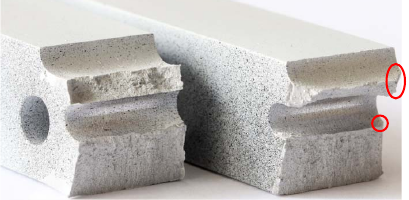
\includegraphics[width=0.9\textwidth,scale=0.5]{Chapter345/figures/split_experiment}
        \end{subfigure}
        \begin{subfigure}[b]{0.45\textwidth}
          \centering
          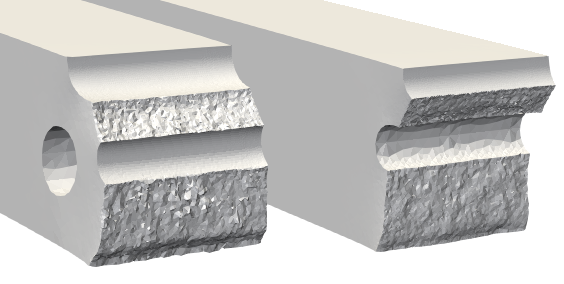
\includegraphics[width=0.9\textwidth,scale=0.5]{Chapter345/figures/split}
        \end{subfigure}
      \end{figure}
    \end{column}
    \begin{column}{0.4\textwidth}
      \begin{itemize}
        \item A \textcolor{peggyblue}{three-point bending} experiment is simulated.
        \item The \textcolor{peggyblue}{aluminum} specimen is modeled as a \textcolor{peggyblue}{compressible Neo-Hookean} material, with \textcolor{peggyblue}{linear hardening}, \textcolor{peggyblue}{$\tqf = 1$}.
        \item \textcolor{peggyblue}{Coalescence dissipation} is included. The effects of $\beta$ and $\varepsilon_0$ are investigated in a 2D setting.
        \item Parameters are calibrated based on a \textcolor{peggyblue}{tensile tension test}.
        \item ``Shear lips'' are not captured by numerical simulations.
        \item Crack paths and load deflection curves have \textcolor{peggyblue}{excellent agreement} with the experiment.
      \end{itemize}
    \end{column}
  \end{columns}
\end{frame}

\begin{frame}
  \vspace{-1.5em}
  \begin{columns}[T]
    \begin{column}{0.6\textwidth}
      \vspace{-1em}
      \begin{figure}
        \centering
        \begin{subfigure}{0.95\linewidth}
          \centering
          \begin{tikzpicture}
            \node[inner sep=0] (mesh) at (0,0) {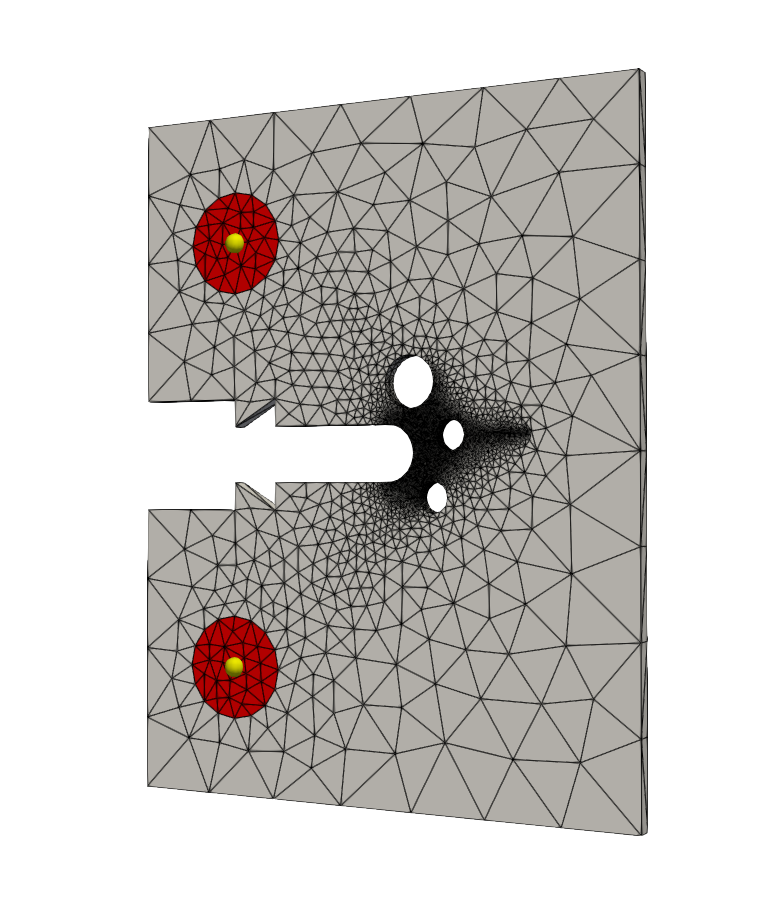
\includegraphics[width=0.3\textwidth,scale=0.5]{Chapter345/figures/mesh}};
            \coordinate (box_sw) at (-0.15, -0.4);
            \coordinate (box_nw) at (-0.15, 0.48);
            \coordinate (box_ne) at (0.5, 0.55);
            \coordinate (box_se) at (0.5, -0.43);
            
            \draw [blue] (box_sw) -- (box_nw);
            \draw [blue] (box_nw) -- (box_ne);
            \draw [blue] (box_ne) -- (box_se);
            \draw [blue] (box_se) -- (box_sw);
            
            \node[inner sep=0] (meshzoom) at (3,0) {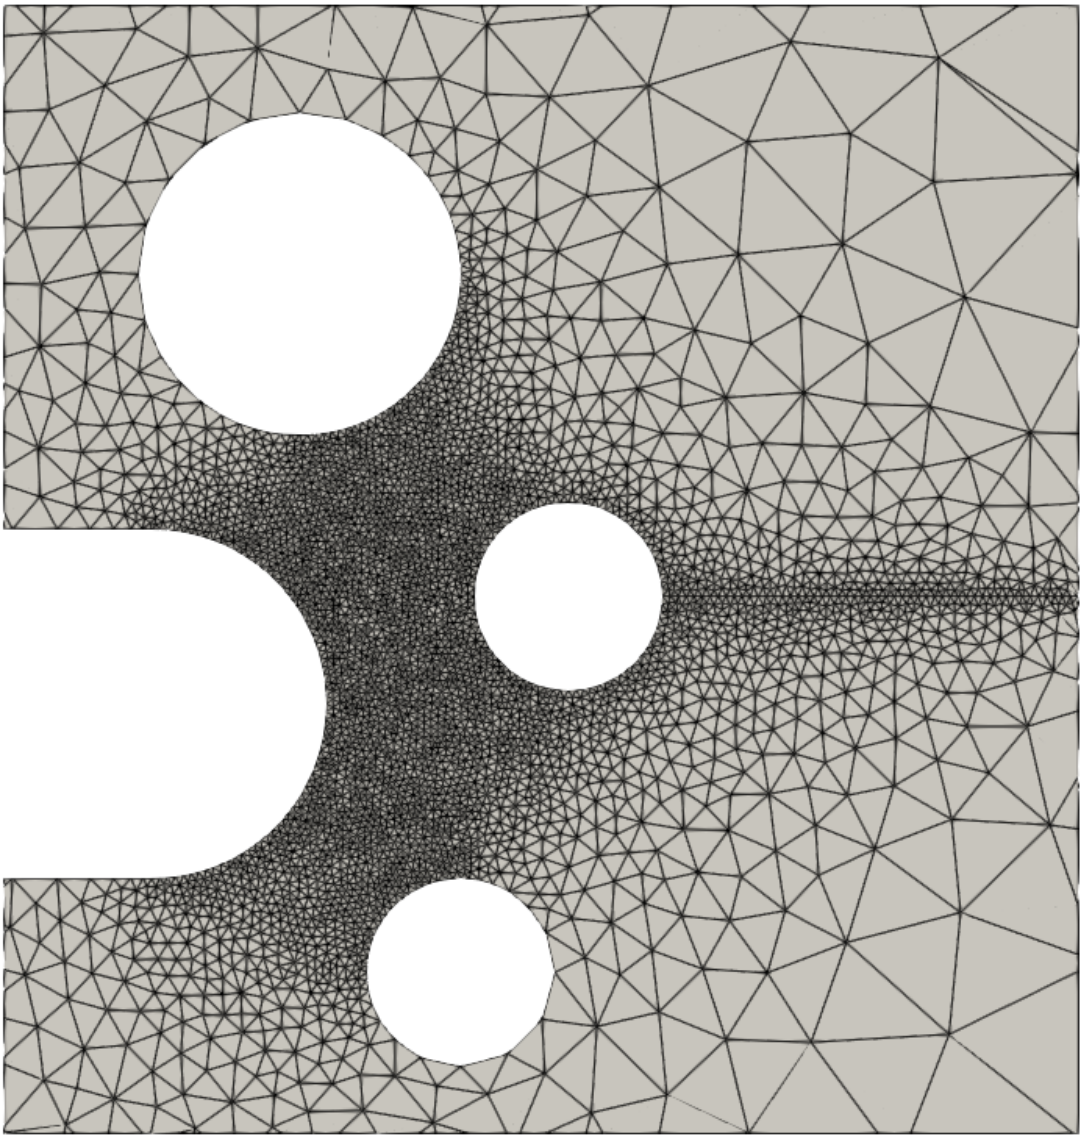
\includegraphics[width=0.3\textwidth,scale=0.5]{Chapter345/figures/meshzoom}};
            \node (boxzoom) at (meshzoom.south west) [draw,blue,thick,minimum width=0.3\textwidth,minimum height=72,anchor=south west] {};
            
            \draw (box_ne) -- (boxzoom.north west);
            \draw (box_se) -- (boxzoom.south west);
            
            \node (A) at (-0.45,0.85) [yellow] {\textbf{A}};
            \node (B) at (-0.45,-0.85) [yellow] {\textbf{B}};
          \end{tikzpicture}
        \end{subfigure}
        
        \begin{subfigure}{0.32\textwidth}
          \centering
          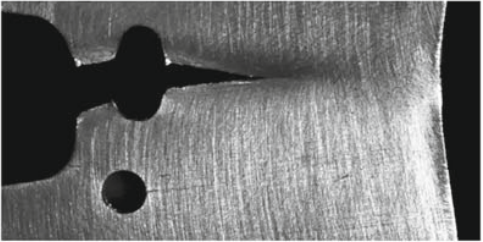
\includegraphics[width=\textwidth]{Chapter345/figures/SFC_schematics}
        \end{subfigure}
        \begin{subfigure}{0.32\textwidth}
          \centering
          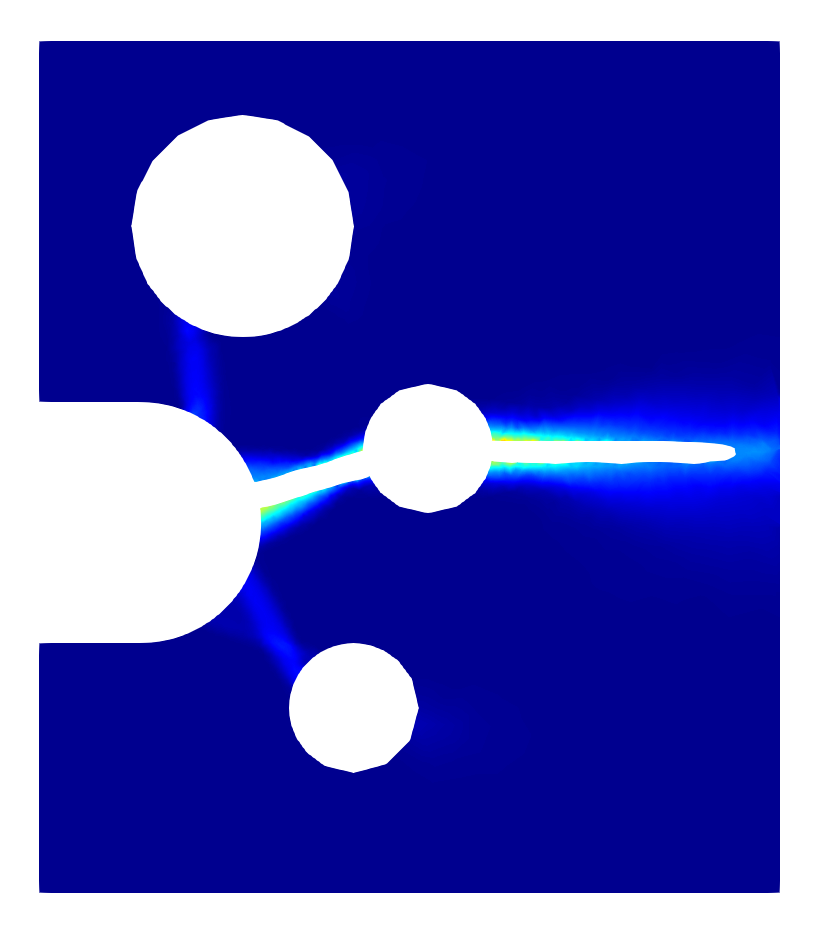
\includegraphics[width=0.55\textwidth]{Chapter345/figures/W_pl_3}
        \end{subfigure}
        \begin{subfigure}{0.32\textwidth}
          \centering
          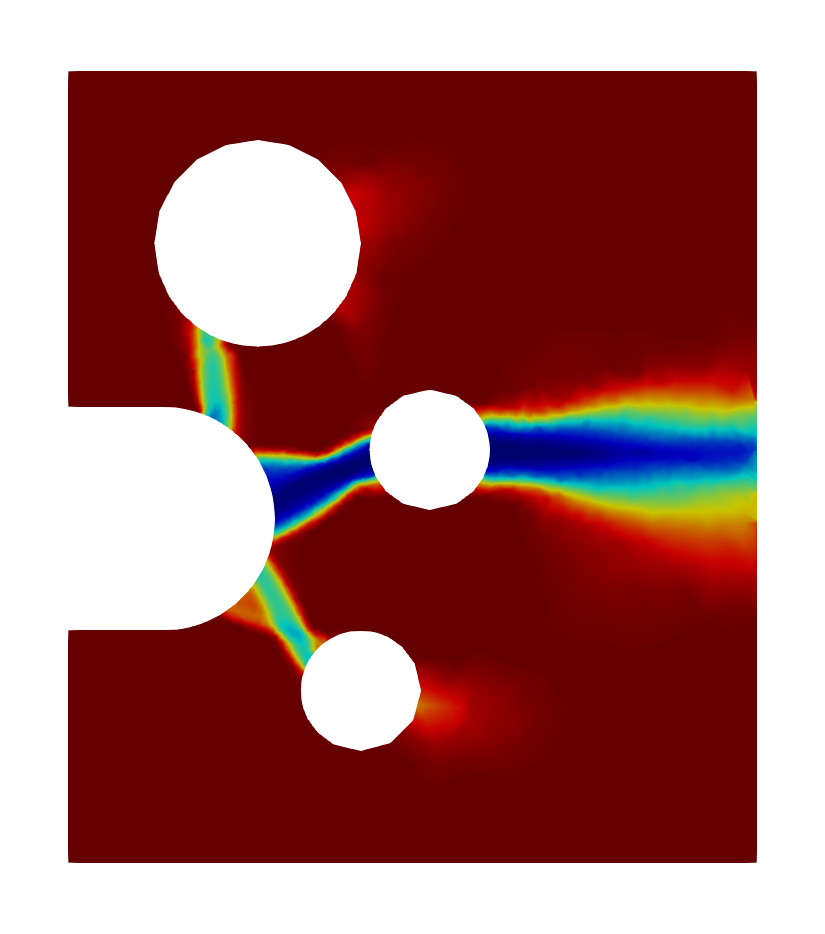
\includegraphics[width=0.62\textwidth]{Chapter345/figures/M_3}
        \end{subfigure}
        
        \begin{subfigure}{0.95\textwidth}
          \begin{tikzpicture}
            \begin{axis}[
                cycle list name=exotic,
                width=\textwidth,
                height=0.4\textwidth,
                xmin=0,xmax=7,
                ymin=0,
                xlabel=displacement(\SI{}{\milli\meter}),ylabel=force(\SI{}{\kilo\newton}),
                scaled y ticks=false,
                xticklabel style={
                    /pgf/number format/fixed,
                    /pgf/number format/precision=2
                  },
                legend style={
                    at={(0.1,0.05)},
                    anchor=south west,
                    nodes={scale=0.6, transform shape},
                    fill=none,
                    draw=none,
                    cells={align=left}
                  },
                legend cell align={left},
                every axis plot/.append style={thick}
              ]
              \addplot +[mark=none,black,dashed] table[x expr=\thisrowno{0},y expr=\thisrowno{1}/1000,col sep=comma]{Chapter345/data/experiment.csv};
              \addplot +[mark=none] table[x expr=\thisrowno{0},y expr=\thisrowno{1}/1000,col sep=comma]{Chapter345/data/force_disp.csv};
              \addplot +[mark=none] table[x expr=\thisrowno{0},y expr=\thisrowno{1}/1000,col sep=comma]{Chapter345/data/force_disp_lorenzis_1.csv};
              \addplot +[mark=none] table[x expr=\thisrowno{0},y expr=\thisrowno{1}/1000,col sep=comma]{Chapter345/data/force_disp_lorenzis_2.csv};
              \legend{experiment,proposed E-P-D model,prediction with $m=1$ from Ambati et al.,prediction with $m=2$ from Ambati et al.}
            \end{axis}
          \end{tikzpicture}
        \end{subfigure}
      \end{figure}
    \end{column}
    \begin{column}{0.4\textwidth}
      \begin{itemize}
        \item A recent \textcolor{peggyblue}{Sandia Fracture Challenge}.
        \item Material properties are calibrated using provided \textcolor{peggyblue}{tensile tension test} data.
        \item Loading pins A and B are modeled as purely elastic materials with the same constants as the specimen.
        \item The predicted \textcolor{peggyblue}{force-displacement curve} is compared with the experimental data and predictions by other existing phase-field models of ductile fracture.
        \item The agreement between the experiment and our simulation is \textcolor{peggyblue}{remarkable}, both in terms of the crack path and the force-displacement curve.
      \end{itemize}
    \end{column}
  \end{columns}
\end{frame}

\begin{frame}
  \begin{columns}[T]
    \begin{column}{0.5\textwidth}
      \begin{figure}
        \centering
        \begin{subfigure}{0.45\textwidth}
          \centering
          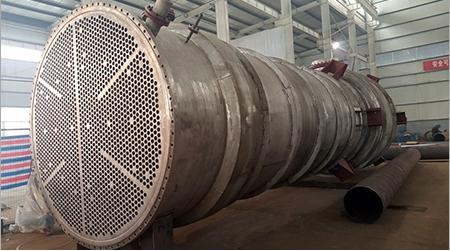
\includegraphics[width=\textwidth]{Chapter345/figures/HTHX}
        \end{subfigure}
        \begin{subfigure}{0.45\textwidth}
          \centering
          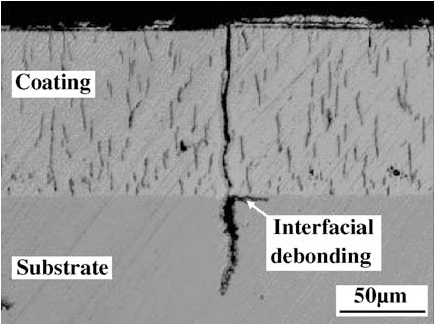
\includegraphics[width=\textwidth]{Chapter345/figures/debonding}
        \end{subfigure}
      \end{figure}
      
      Background:
      \begin{itemize}
        \item \textcolor{peggyblue}{High temperature heat exchangers} are key components of many power conversion systems, including advanced nuclear power generation systems.
        \item They operate in the inlet temperature range of 750-1100 \SI{}{\celsius} and are subject to unique operating challenges including \textcolor{peggyblue}{oxidation}, \textcolor{peggyblue}{corrosion}, \textcolor{peggyblue}{creep} and \textcolor{peggyblue}{fracture}.
      \end{itemize}
    \end{column}
    \begin{column}{0.5\textwidth}
      Model:
      \begin{itemize}
        \item To model energy release associated with debonding:
              \begin{align*}
                \psi^f = \dfrac{\Gc}{c_0 l} \left( C\alpha(d) + l^2 \grad d \cdot \grad d \right) + \textcolor{peggyblue}{\dfrac{1}{\tau} \mathcal{G} \omega(c)}.
              \end{align*}
        \item A lower dimensional representation of the oxide layer:
              \begin{align*}
                \psi^e & =  g^e_\text{ip} \psi^e_{\text{ip}, \activepart} + \psi^e_{\text{ip}, \inactivepart} + g^e_\text{op} \psi^e_{\text{op}, \activepart} + \psi^e_{\text{ip}, \inactivepart}. 
              \end{align*}
        \item The perfect plasticity model with thermal softening is approximated using a power-law creep model:
              \begin{align*}
                \epdot = A \left( \dfrac{\bar{\sigma}}{g^p \sigma_0} \right)^n \exp\left( -\dfrac{nQ}{RT} \right).
              \end{align*}
      \end{itemize}
    \end{column}
  \end{columns}
\end{frame}

\begin{frame}
  \vspace{-1.5em}
  \begin{columns}[T]
    \begin{column}{0.6\textwidth}
      \vspace{-1.5em}
      \begin{figure}
        \centering
        \only<1>{
          \begin{subfigure}{0.3\textwidth}
            \centering
            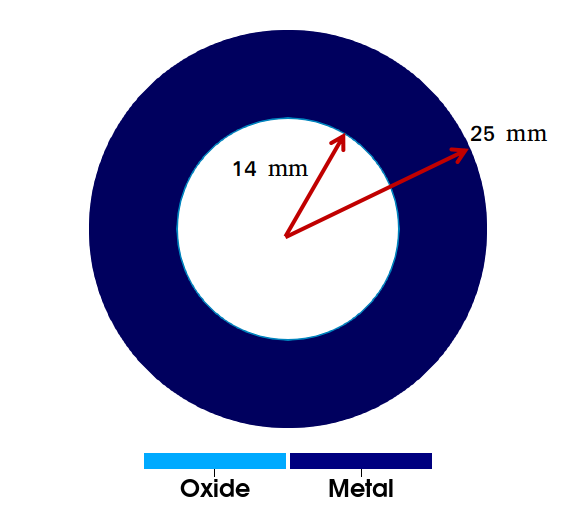
\includegraphics[width=\textwidth]{Chapter345/figures/top_view}
          \end{subfigure}
          \hspace{0.1\textwidth}
          \begin{subfigure}{0.3\textwidth}
            \centering
            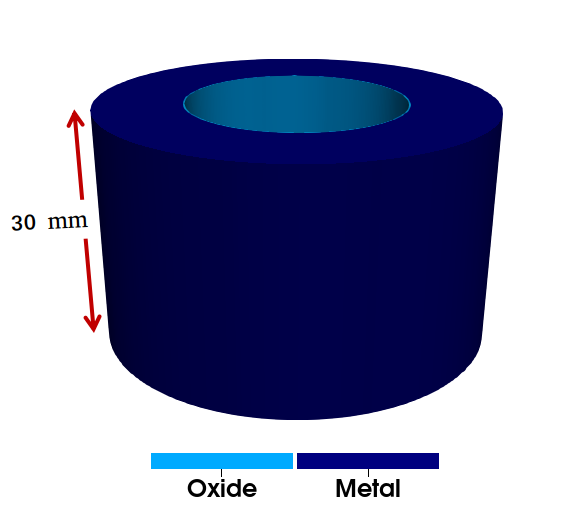
\includegraphics[width=\textwidth]{Chapter345/figures/side_view}
          \end{subfigure}
          
          \begin{subfigure}{0.4\textwidth}
            \centering
            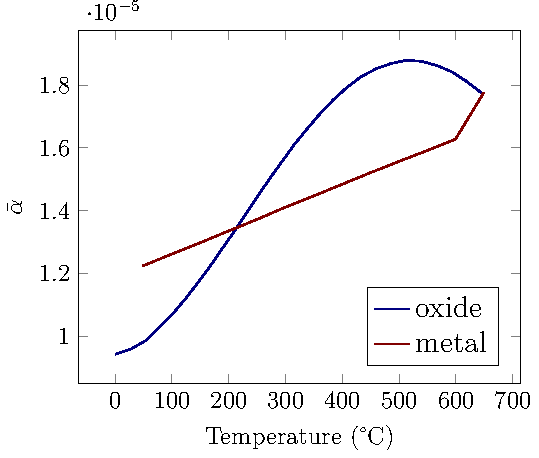
\includegraphics[width=0.8\textwidth]{Chapter345/figures/CTE}
          \end{subfigure}
          \begin{subfigure}{0.4\textwidth}
            \centering
            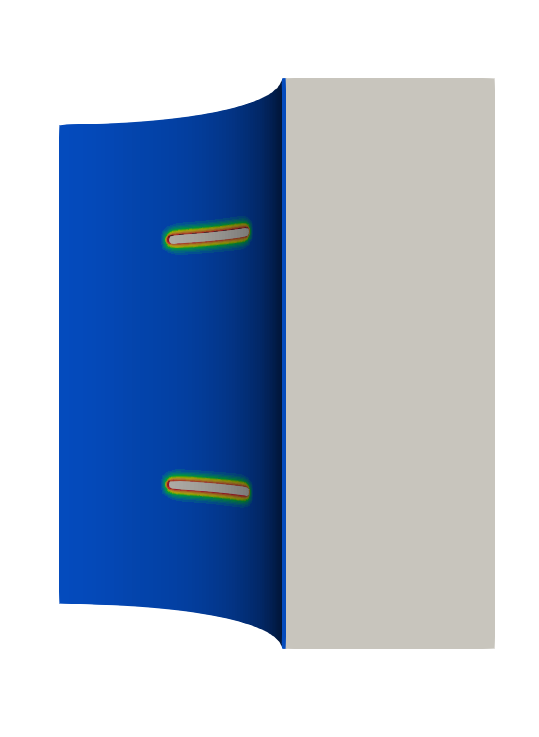
\includegraphics[width=0.5\textwidth]{Chapter345/figures/seed_d_1}
          \end{subfigure}
          
          \begin{subfigure}{0.25\textwidth}
            \centering
            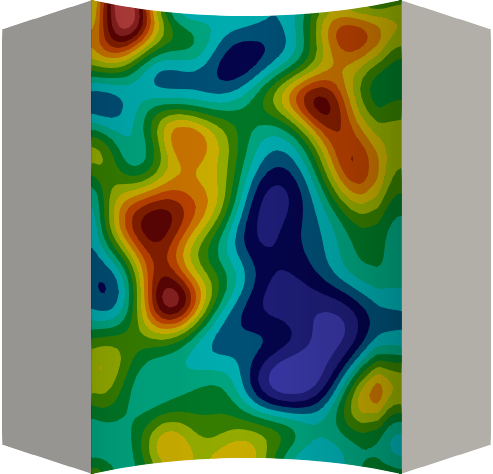
\includegraphics[width=\textwidth]{Chapter345/figures/E.0000}
          \end{subfigure}
          \begin{subfigure}{0.1\textwidth}
            \centering
            \caption*{$E/\underline{E}$}
            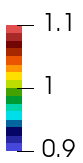
\includegraphics[width=\textwidth]{Chapter345/figures/colorbar_rf}
          \end{subfigure}
          \hspace{0.1\textwidth}
          \begin{subfigure}{0.25\textwidth}
            \centering
            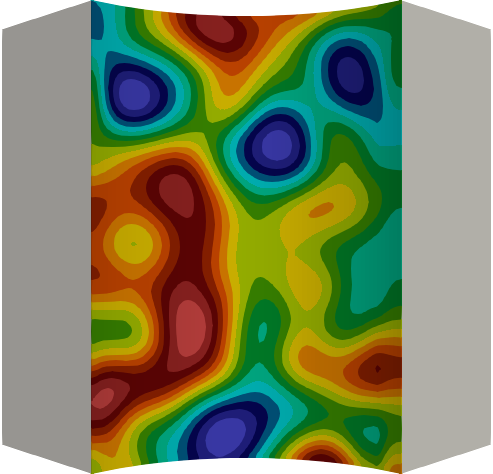
\includegraphics[width=\textwidth]{Chapter345/figures/Gc.0000}
          \end{subfigure}
          \begin{subfigure}{0.1\textwidth}
            \centering
            \caption*{$\Gc/\underline{\Gc}$}
            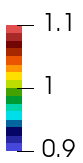
\includegraphics[width=\textwidth]{Chapter345/figures/colorbar_rf}
          \end{subfigure}
        }
        
        \only<2->{
          \begin{subfigure}{\textwidth}
            \caption*{Case I: Initial transverse cracks}
          \end{subfigure}
          
          \vspace{-1em}
          
          \begin{subfigure}{0.15\textwidth}
            \caption*{}
          \end{subfigure}
          \begin{subfigure}{0.19\textwidth}
            \centering
            \caption*{$c$}
          \end{subfigure}
          \hspace{0.06\textwidth}
          \begin{subfigure}{0.19\textwidth}
            \centering
            \caption*{$d$}
          \end{subfigure}
          \hspace{0.06\textwidth}
          \begin{subfigure}{0.19\textwidth}
            \centering
            \caption*{$\ep$}
          \end{subfigure}
          
          \vspace{-1em}
          
          \begin{subfigure}{0.15\textwidth}
            \caption*{}
          \end{subfigure}
          \begin{subfigure}{0.19\textwidth}
            \centering
            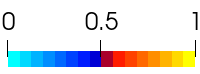
\includegraphics[width=\textwidth]{Chapter345/figures/colorbar_c_rf}
          \end{subfigure}
          \hspace{0.06\textwidth}
          \begin{subfigure}{0.19\textwidth}
            \centering
            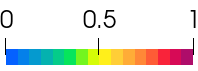
\includegraphics[width=\textwidth]{Chapter345/figures/colorbar_d_rf}
          \end{subfigure}
          \hspace{0.06\textwidth}
          \begin{subfigure}{0.19\textwidth}
            \centering
            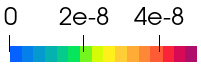
\includegraphics[width=\textwidth]{Chapter345/figures/colorbar_ep_rf}
          \end{subfigure}
        }
        
        \only<2>{
          \begin{subfigure}{0.15\textwidth}
            \centering
            \caption*{0 day}
          \end{subfigure}
          \begin{subfigure}{0.19\textwidth}
            \centering
            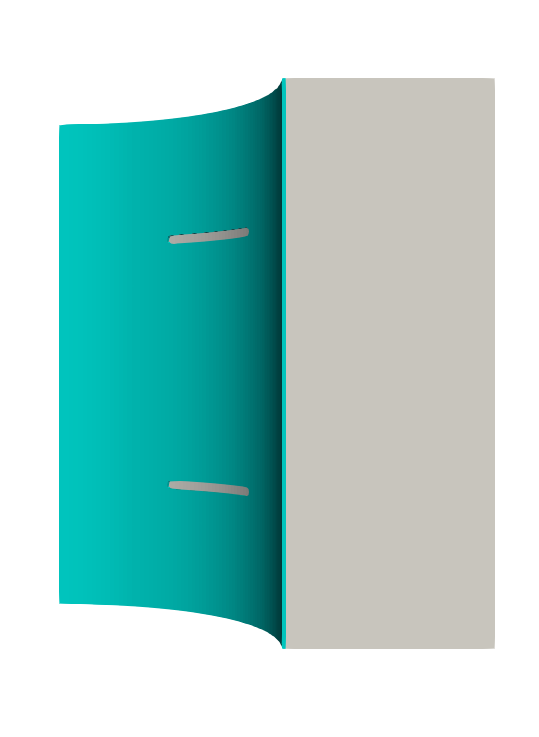
\includegraphics[width=\textwidth]{Chapter345/figures/seed_c_1}
          \end{subfigure}
          \hspace{0.06\textwidth}
          \begin{subfigure}{0.19\textwidth}
            \centering
            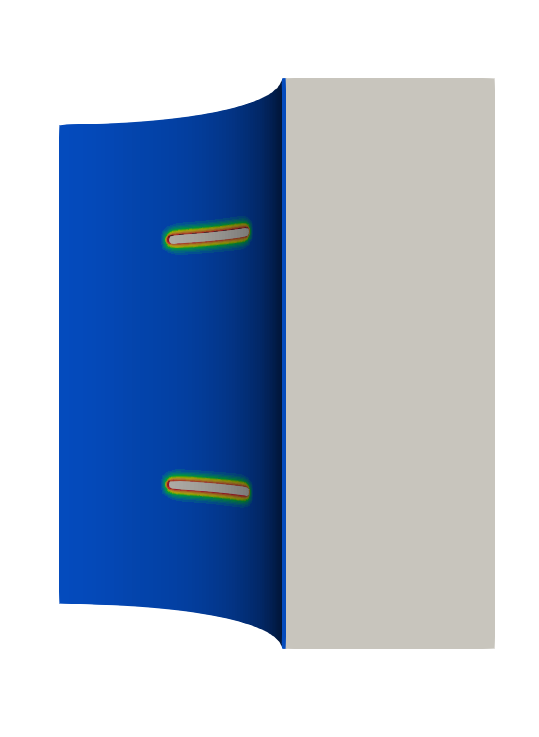
\includegraphics[width=\textwidth]{Chapter345/figures/seed_d_1}
          \end{subfigure}
          \hspace{0.06\textwidth}
          \begin{subfigure}{0.19\textwidth}
            \centering
            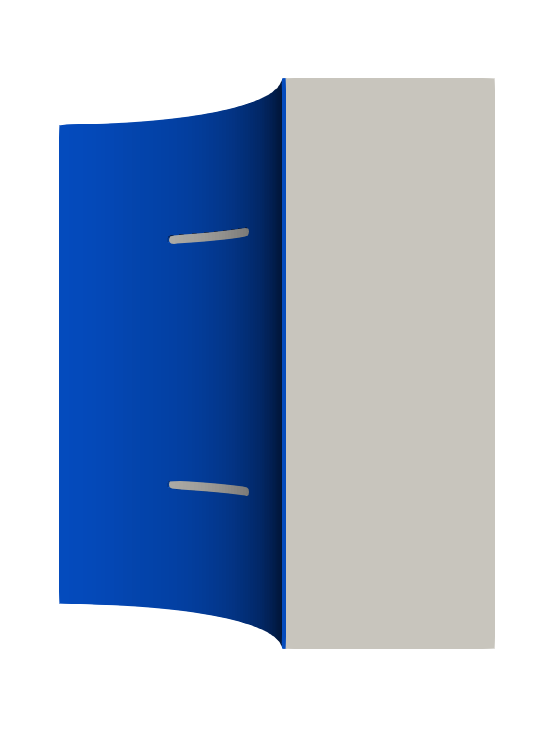
\includegraphics[width=\textwidth]{Chapter345/figures/seed_ep_1}
          \end{subfigure}
        }
        
        \only<3>{
          \begin{subfigure}{0.15\textwidth}
            \centering
            \caption*{60 days}
          \end{subfigure}
          \begin{subfigure}{0.19\textwidth}
            \centering
            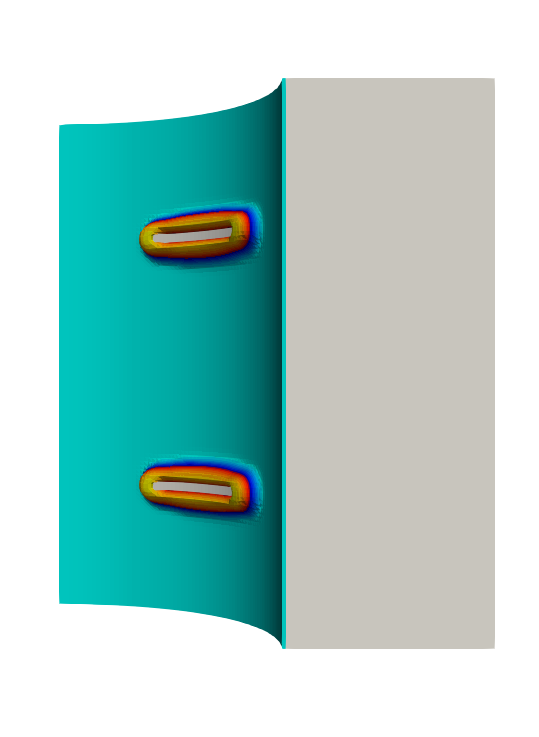
\includegraphics[width=\textwidth]{Chapter345/figures/seed_c_2}
          \end{subfigure}
          \hspace{0.06\textwidth}
          \begin{subfigure}{0.19\textwidth}
            \centering
            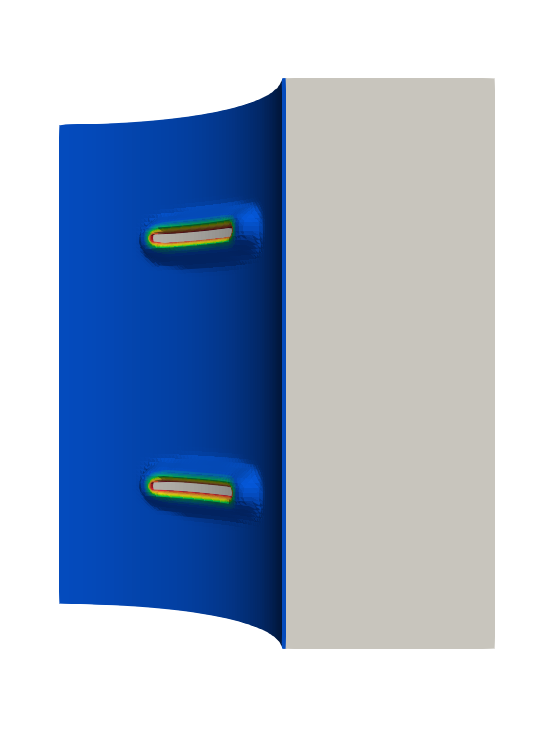
\includegraphics[width=\textwidth]{Chapter345/figures/seed_d_2}
          \end{subfigure}
          \hspace{0.06\textwidth}
          \begin{subfigure}{0.19\textwidth}
            \centering
            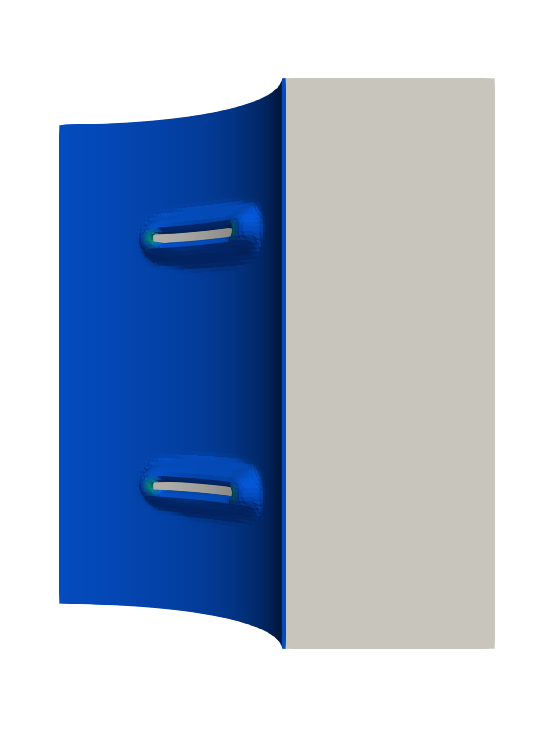
\includegraphics[width=\textwidth]{Chapter345/figures/seed_ep_2}
          \end{subfigure}
        }
        
        \only<4>{
          \begin{subfigure}{0.15\textwidth}
            \centering
            \caption*{120 days}
          \end{subfigure}
          \begin{subfigure}{0.19\textwidth}
            \centering
            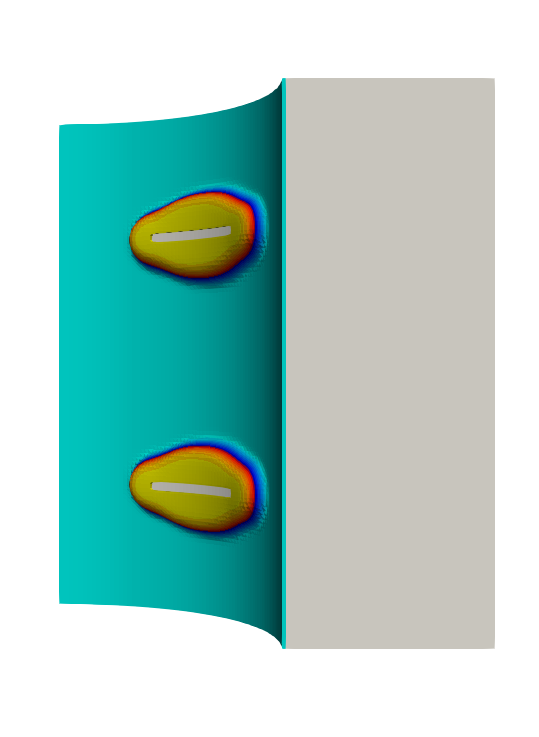
\includegraphics[width=\textwidth]{Chapter345/figures/seed_c_3}
          \end{subfigure}
          \hspace{0.06\textwidth}
          \begin{subfigure}{0.19\textwidth}
            \centering
            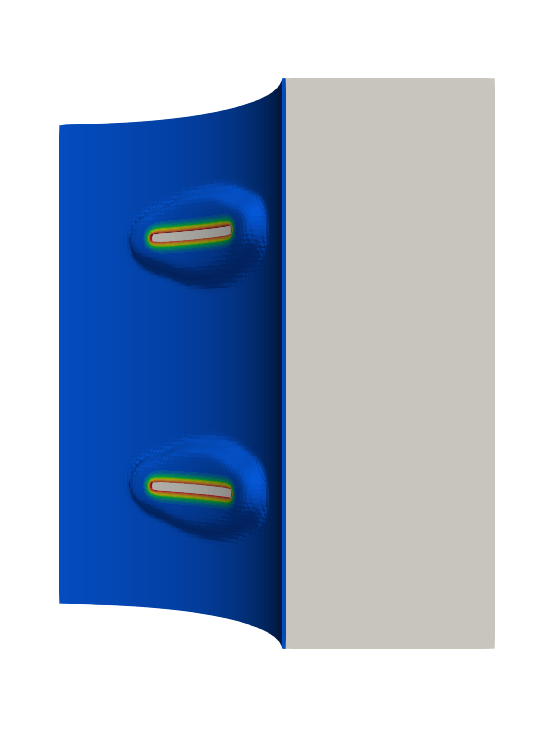
\includegraphics[width=\textwidth]{Chapter345/figures/seed_d_3}
          \end{subfigure}
          \hspace{0.06\textwidth}
          \begin{subfigure}{0.19\textwidth}
            \centering
            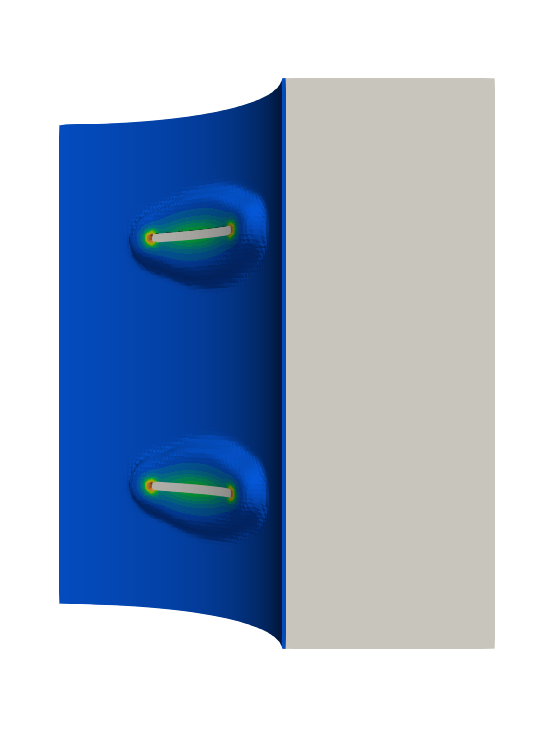
\includegraphics[width=\textwidth]{Chapter345/figures/seed_ep_3}
          \end{subfigure}
        }
        
        \only<5>{
          \begin{subfigure}{0.15\textwidth}
            \centering
            \caption*{180 days}
          \end{subfigure}
          \begin{subfigure}{0.19\textwidth}
            \centering
            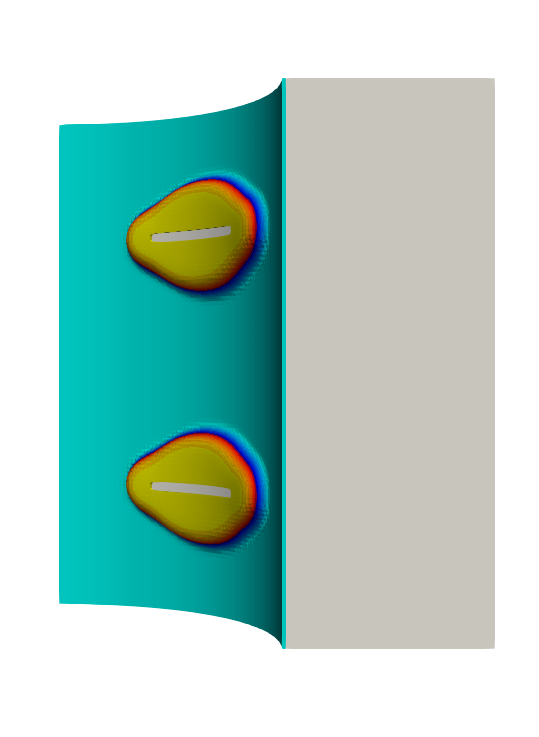
\includegraphics[width=\textwidth]{Chapter345/figures/seed_c_4}
          \end{subfigure}
          \hspace{0.06\textwidth}
          \begin{subfigure}{0.19\textwidth}
            \centering
            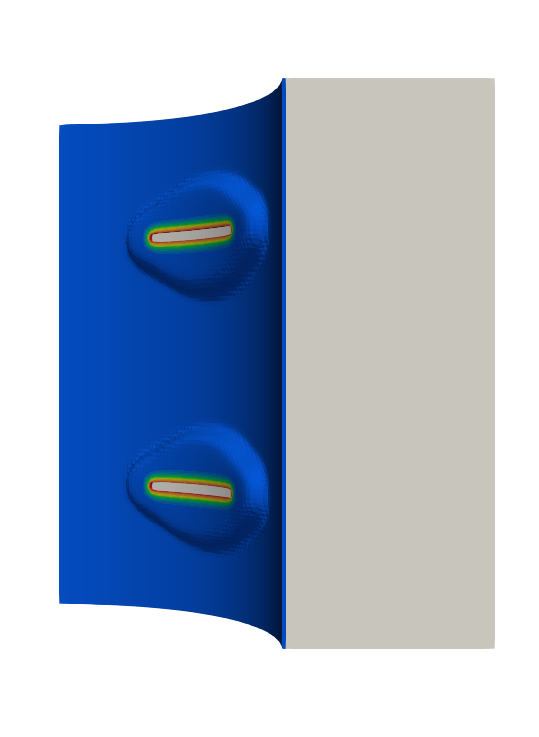
\includegraphics[width=\textwidth]{Chapter345/figures/seed_d_4}
          \end{subfigure}
          \hspace{0.06\textwidth}
          \begin{subfigure}{0.19\textwidth}
            \centering
            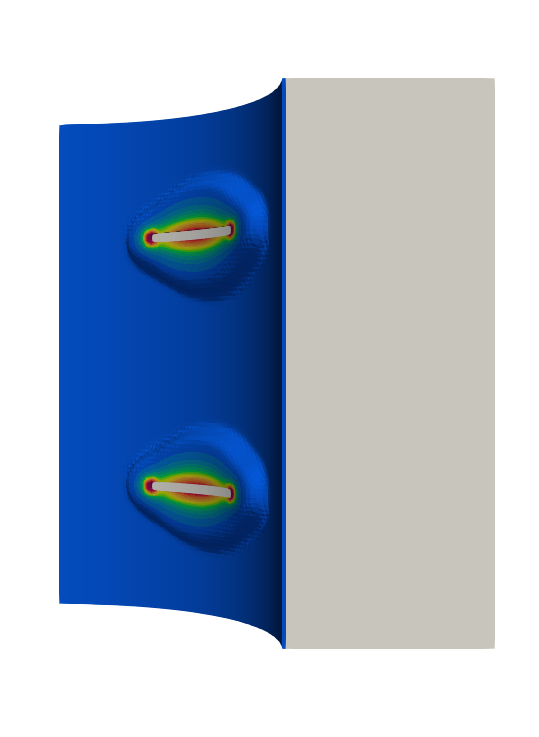
\includegraphics[width=\textwidth]{Chapter345/figures/seed_ep_4}
          \end{subfigure}
        }
        
        \only<6>{
          \begin{subfigure}{0.15\textwidth}
            \centering
            \caption*{1 hour}
          \end{subfigure}
          \begin{subfigure}{0.19\textwidth}
            \centering
            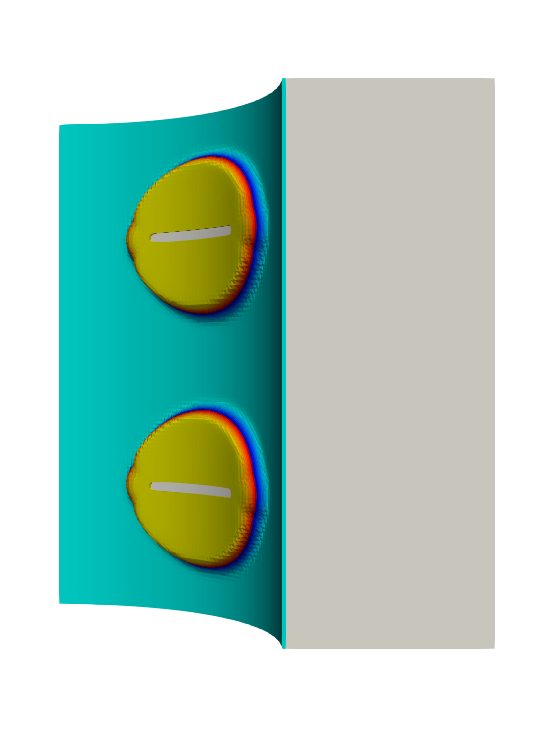
\includegraphics[width=\textwidth]{Chapter345/figures/seed_c_5}
          \end{subfigure}
          \hspace{0.06\textwidth}
          \begin{subfigure}{0.19\textwidth}
            \centering
            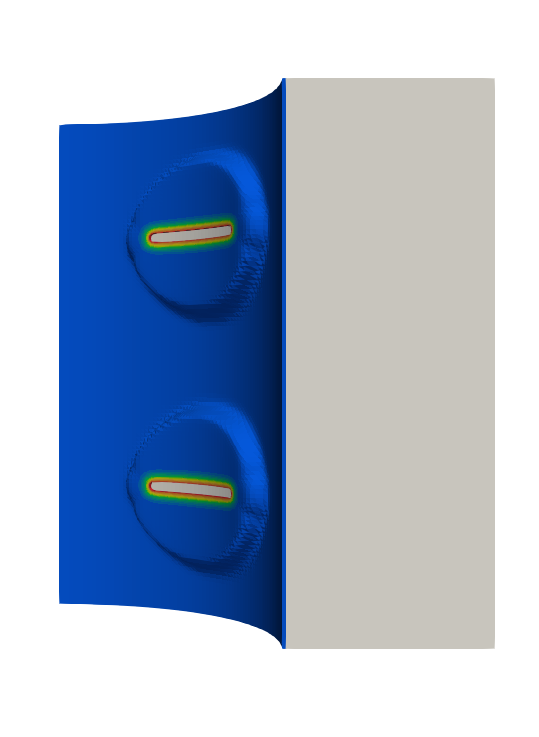
\includegraphics[width=\textwidth]{Chapter345/figures/seed_d_5}
          \end{subfigure}
          \hspace{0.06\textwidth}
          \begin{subfigure}{0.19\textwidth}
            \centering
            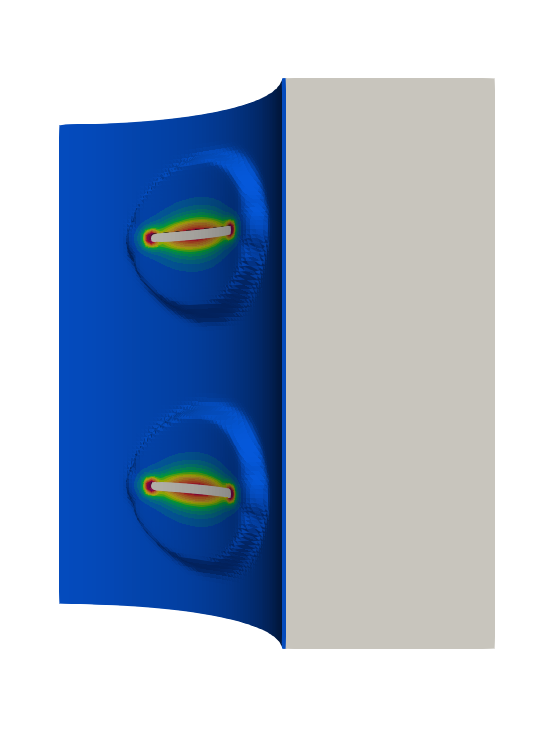
\includegraphics[width=\textwidth]{Chapter345/figures/seed_ep_5}
          \end{subfigure}
        }
        
        \only<7>{
          \begin{subfigure}{0.15\textwidth}
            \centering
            \caption*{2 hours}
          \end{subfigure}
          \begin{subfigure}{0.19\textwidth}
            \centering
            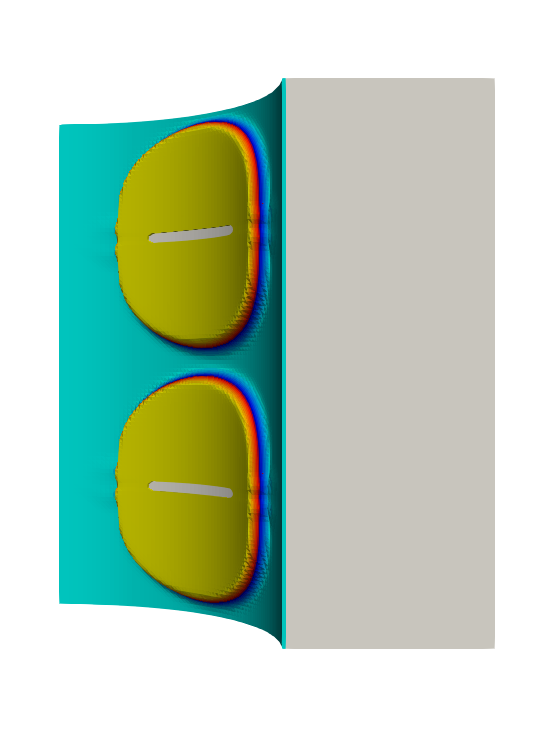
\includegraphics[width=\textwidth]{Chapter345/figures/seed_c_6}
          \end{subfigure}
          \hspace{0.06\textwidth}
          \begin{subfigure}{0.19\textwidth}
            \centering
            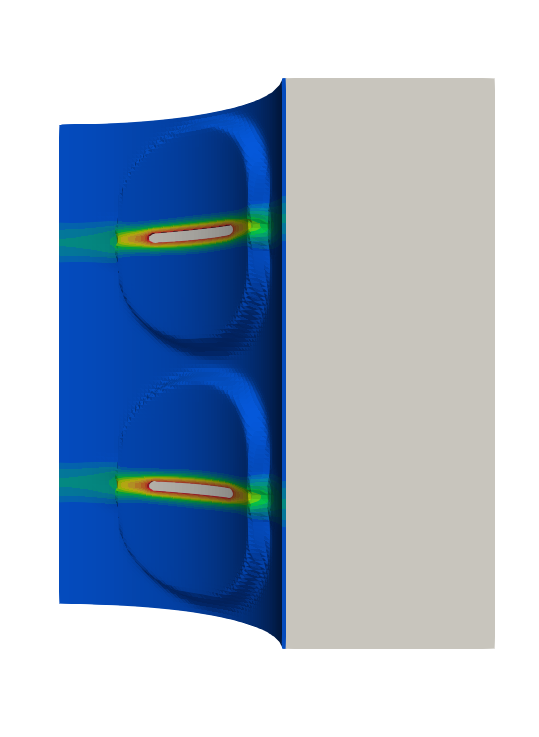
\includegraphics[width=\textwidth]{Chapter345/figures/seed_d_6}
          \end{subfigure}
          \hspace{0.06\textwidth}
          \begin{subfigure}{0.19\textwidth}
            \centering
            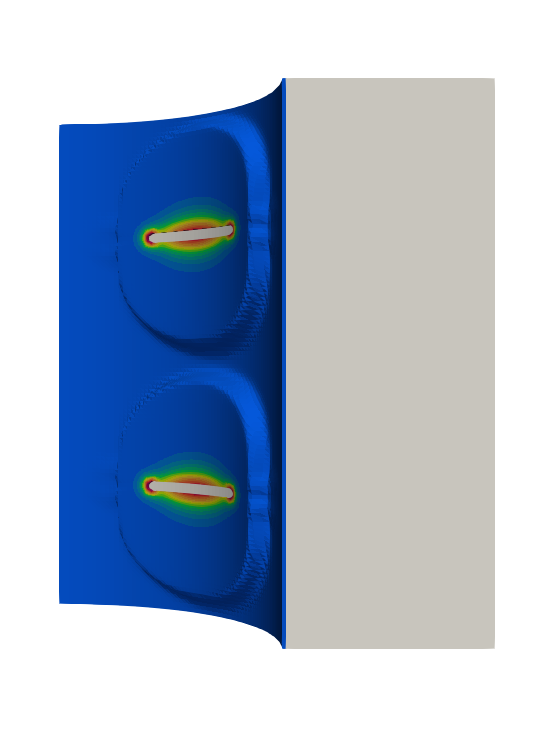
\includegraphics[width=\textwidth]{Chapter345/figures/seed_ep_6}
          \end{subfigure}
        }
        
        \only<8->{
          \begin{subfigure}{0.15\textwidth}
            \centering
            \caption*{3 hours}
          \end{subfigure}
          \begin{subfigure}{0.19\textwidth}
            \centering
            \includegraphics[width=\textwidth]{Chapter345/figures/seed_c_7}
          \end{subfigure}
          \hspace{0.06\textwidth}
          \begin{subfigure}{0.19\textwidth}
            \centering
            \includegraphics[width=\textwidth]{Chapter345/figures/seed_d_7}
          \end{subfigure}
          \hspace{0.06\textwidth}
          \begin{subfigure}{0.19\textwidth}
            \centering
            \includegraphics[width=\textwidth]{Chapter345/figures/seed_ep_7}
          \end{subfigure}
        }
        
        \only<9->{
          \begin{subfigure}{\textwidth}
            \caption*{Case II: Inhomogeneous Young's modulus and Fracture toughness}
          \end{subfigure}
          
          \vspace{-1em}
          
          \begin{subfigure}{0.15\textwidth}
            \caption*{}
          \end{subfigure}
          \begin{subfigure}{0.19\textwidth}
            \centering
            \caption*{$c$}
          \end{subfigure}
          \hspace{0.06\textwidth}
          \begin{subfigure}{0.19\textwidth}
            \centering
            \caption*{$d$}
          \end{subfigure}
          \hspace{0.06\textwidth}
          \begin{subfigure}{0.19\textwidth}
            \centering
            \caption*{$\ep$}
          \end{subfigure}
          
          \vspace{-1em}
          
          \begin{subfigure}{0.15\textwidth}
            \caption*{}
          \end{subfigure}
          \begin{subfigure}{0.19\textwidth}
            \centering
            \includegraphics[width=\textwidth]{Chapter345/figures/colorbar_c_rf}
          \end{subfigure}
          \hspace{0.06\textwidth}
          \begin{subfigure}{0.19\textwidth}
            \centering
            \includegraphics[width=\textwidth]{Chapter345/figures/colorbar_d_rf}
          \end{subfigure}
          \hspace{0.06\textwidth}
          \begin{subfigure}{0.19\textwidth}
            \centering
            \includegraphics[width=\textwidth]{Chapter345/figures/colorbar_ep_rf}
          \end{subfigure}
        }
        
        \only<9>{
          \begin{subfigure}{0.15\textwidth}
            \centering
            \caption*{30 days}
          \end{subfigure}
          \begin{subfigure}{0.19\textwidth}
            \centering
            \includegraphics[width=\textwidth]{Chapter345/figures/c.0003}
          \end{subfigure}
          \hspace{0.06\textwidth}
          \begin{subfigure}{0.19\textwidth}
            \centering
            \includegraphics[width=\textwidth]{Chapter345/figures/d.0003}
          \end{subfigure}
          \hspace{0.06\textwidth}
          \begin{subfigure}{0.19\textwidth}
            \centering
            \includegraphics[width=\textwidth]{Chapter345/figures/ep.0003}
          \end{subfigure}
        }
        
        \only<10>{
          \begin{subfigure}{0.15\textwidth}
            \centering
            \caption*{60 days}
          \end{subfigure}
          \begin{subfigure}{0.19\textwidth}
            \centering
            \includegraphics[width=\textwidth]{Chapter345/figures/c.0006}
          \end{subfigure}
          \hspace{0.06\textwidth}
          \begin{subfigure}{0.19\textwidth}
            \centering
            \includegraphics[width=\textwidth]{Chapter345/figures/d.0006}
          \end{subfigure}
          \hspace{0.06\textwidth}
          \begin{subfigure}{0.19\textwidth}
            \centering
            \includegraphics[width=\textwidth]{Chapter345/figures/ep.0006}
          \end{subfigure}
        }
        
        \only<11>{
          \begin{subfigure}{0.15\textwidth}
            \centering
            \caption*{90 days}
          \end{subfigure}
          \begin{subfigure}{0.19\textwidth}
            \centering
            \includegraphics[width=\textwidth]{Chapter345/figures/c.0009}
          \end{subfigure}
          \hspace{0.06\textwidth}
          \begin{subfigure}{0.19\textwidth}
            \centering
            \includegraphics[width=\textwidth]{Chapter345/figures/d.0009}
          \end{subfigure}
          \hspace{0.06\textwidth}
          \begin{subfigure}{0.19\textwidth}
            \centering
            \includegraphics[width=\textwidth]{Chapter345/figures/ep.0009}
          \end{subfigure}
        }
        
        \only<12>{
          \begin{subfigure}{0.15\textwidth}
            \centering
            \caption*{120 days}
          \end{subfigure}
          \begin{subfigure}{0.19\textwidth}
            \centering
            \includegraphics[width=\textwidth]{Chapter345/figures/c.0012}
          \end{subfigure}
          \hspace{0.06\textwidth}
          \begin{subfigure}{0.19\textwidth}
            \centering
            \includegraphics[width=\textwidth]{Chapter345/figures/d.0012}
          \end{subfigure}
          \hspace{0.06\textwidth}
          \begin{subfigure}{0.19\textwidth}
            \centering
            \includegraphics[width=\textwidth]{Chapter345/figures/ep.0012}
          \end{subfigure}
        }
        
        \only<13>{
          \begin{subfigure}{0.15\textwidth}
            \centering
            \caption*{150 days}
          \end{subfigure}
          \begin{subfigure}{0.19\textwidth}
            \centering
            \includegraphics[width=\textwidth]{Chapter345/figures/c.0015}
          \end{subfigure}
          \hspace{0.06\textwidth}
          \begin{subfigure}{0.19\textwidth}
            \centering
            \includegraphics[width=\textwidth]{Chapter345/figures/d.0015}
          \end{subfigure}
          \hspace{0.06\textwidth}
          \begin{subfigure}{0.19\textwidth}
            \centering
            \includegraphics[width=\textwidth]{Chapter345/figures/ep.0015}
          \end{subfigure}
        }
        
        \only<14>{
          \begin{subfigure}{0.15\textwidth}
            \centering
            \caption*{180 days}
          \end{subfigure}
          \begin{subfigure}{0.19\textwidth}
            \centering
            \includegraphics[width=\textwidth]{Chapter345/figures/c.0018}
          \end{subfigure}
          \hspace{0.06\textwidth}
          \begin{subfigure}{0.19\textwidth}
            \centering
            \includegraphics[width=\textwidth]{Chapter345/figures/d.0018}
          \end{subfigure}
          \hspace{0.06\textwidth}
          \begin{subfigure}{0.19\textwidth}
            \centering
            \includegraphics[width=\textwidth]{Chapter345/figures/ep.0018}
          \end{subfigure}
        }
        
        \only<15>{
          \begin{subfigure}{0.15\textwidth}
            \centering
            \caption*{1 hour}
          \end{subfigure}
          \begin{subfigure}{0.19\textwidth}
            \centering
            \includegraphics[width=\textwidth]{Chapter345/figures/c.0021}
          \end{subfigure}
          \hspace{0.06\textwidth}
          \begin{subfigure}{0.19\textwidth}
            \centering
            \includegraphics[width=\textwidth]{Chapter345/figures/d.0021}
          \end{subfigure}
          \hspace{0.06\textwidth}
          \begin{subfigure}{0.19\textwidth}
            \centering
            \includegraphics[width=\textwidth]{Chapter345/figures/ep.0021}
          \end{subfigure}
        }
        
        \only<16>{
          \begin{subfigure}{0.15\textwidth}
            \centering
            \caption*{2 hours}
          \end{subfigure}
          \begin{subfigure}{0.19\textwidth}
            \centering
            \includegraphics[width=\textwidth]{Chapter345/figures/c.0024}
          \end{subfigure}
          \hspace{0.06\textwidth}
          \begin{subfigure}{0.19\textwidth}
            \centering
            \includegraphics[width=\textwidth]{Chapter345/figures/d.0024}
          \end{subfigure}
          \hspace{0.06\textwidth}
          \begin{subfigure}{0.19\textwidth}
            \centering
            \includegraphics[width=\textwidth]{Chapter345/figures/ep.0024}
          \end{subfigure}
        }
        
        \only<17>{
          \begin{subfigure}{0.15\textwidth}
            \centering
            \caption*{3 hours}
          \end{subfigure}
          \begin{subfigure}{0.19\textwidth}
            \centering
            \includegraphics[width=\textwidth]{Chapter345/figures/c.0027}
          \end{subfigure}
          \hspace{0.06\textwidth}
          \begin{subfigure}{0.19\textwidth}
            \centering
            \includegraphics[width=\textwidth]{Chapter345/figures/d.0027}
          \end{subfigure}
          \hspace{0.06\textwidth}
          \begin{subfigure}{0.19\textwidth}
            \centering
            \includegraphics[width=\textwidth]{Chapter345/figures/ep.0027}
          \end{subfigure}
        }
        
        \only<18>{
          \begin{subfigure}{0.15\textwidth}
            \centering
            \caption*{4 hours}
          \end{subfigure}
          \begin{subfigure}{0.19\textwidth}
            \centering
            \includegraphics[width=\textwidth]{Chapter345/figures/c.0030}
          \end{subfigure}
          \hspace{0.06\textwidth}
          \begin{subfigure}{0.19\textwidth}
            \centering
            \includegraphics[width=\textwidth]{Chapter345/figures/d.0030}
          \end{subfigure}
          \hspace{0.06\textwidth}
          \begin{subfigure}{0.19\textwidth}
            \centering
            \includegraphics[width=\textwidth]{Chapter345/figures/ep.0030}
          \end{subfigure}
        }
        
        \only<19>{
          \begin{subfigure}{0.15\textwidth}
            \centering
            \caption*{5 hours}
          \end{subfigure}
          \begin{subfigure}{0.19\textwidth}
            \centering
            \includegraphics[width=\textwidth]{Chapter345/figures/c.0033}
          \end{subfigure}
          \hspace{0.06\textwidth}
          \begin{subfigure}{0.19\textwidth}
            \centering
            \includegraphics[width=\textwidth]{Chapter345/figures/d.0033}
          \end{subfigure}
          \hspace{0.06\textwidth}
          \begin{subfigure}{0.19\textwidth}
            \centering
            \includegraphics[width=\textwidth]{Chapter345/figures/ep.0033}
          \end{subfigure}
        }
        
        \only<20>{
          \begin{subfigure}{0.15\textwidth}
            \centering
            \caption*{6 hours}
          \end{subfigure}
          \begin{subfigure}{0.19\textwidth}
            \centering
            \includegraphics[width=\textwidth]{Chapter345/figures/c.0036}
          \end{subfigure}
          \hspace{0.06\textwidth}
          \begin{subfigure}{0.19\textwidth}
            \centering
            \includegraphics[width=\textwidth]{Chapter345/figures/d.0036}
          \end{subfigure}
          \hspace{0.06\textwidth}
          \begin{subfigure}{0.19\textwidth}
            \centering
            \includegraphics[width=\textwidth]{Chapter345/figures/ep.0036}
          \end{subfigure}
        }
      \end{figure}
    \end{column}
    \begin{column}{0.4\textwidth}
      \begin{itemize}
        \item The HTHX is simulated for 180 days under \textcolor{peggyblue}{normal operating conditions}, followed by a \textcolor{peggyblue}{shutdown} (6-hour transition).
        \item The HTHX is surround by \textcolor{peggyblue}{high temperature pressurized} fluids during normal operation. The temperature and the pressure of the fluids drop after shutting down.
        \item Most model parameters are adopted from \cite{xue2020stress}.
        \item[\textcolor{peggyblue}{\textbullet}] Creep deformation accumulates under normal operating conditions. The effective creep strain localizes around the cracks.
        \item[\textcolor{peggyblue}{\textbullet}] Debonding occurs at weaker locations in the vicinity of the crack surfaces.
        \item[\textcolor{peggyblue}{\textbullet}] Transverse cracks nucleate and propagate while shutting down.
      \end{itemize}
    \end{column}
  \end{columns}
\end{frame}
